\documentclass[paper=a4, fontsize=11pt]{scrartcl}
\usepackage[T1]{fontenc}
\usepackage{fourier}

\usepackage[english]{babel}															% English language/hyphenation
\usepackage[protrusion=true,expansion=true]{microtype}	
\usepackage{amsmath,amsfonts,amsthm} % Math packages
\usepackage[pdftex]{graphicx}	
\usepackage{url}
\usepackage{hyperref}


%%% Custom sectioning
\usepackage{sectsty}
\allsectionsfont{\centering \normalfont\scshape}
\usepackage{subfigure}
\usepackage{comment}


%%% Custom headers/footers (fancyhdr package)
\usepackage{fancyhdr}
\pagestyle{fancyplain}
\fancyhead{}											% No page header
\fancyfoot[L]{}											% Empty 
\fancyfoot[C]{}											% Empty
\fancyfoot[R]{\thepage}									% Pagenumbering
\renewcommand{\headrulewidth}{0pt}			% Remove header underlines
\renewcommand{\footrulewidth}{0pt}				% Remove footer underlines
\setlength{\headheight}{13.6pt}


%%% Equation and float numbering
%\numberwithin{equation}{section}		% Equationnumbering: section.eq#
%\numberwithin{figure}{section}			% Figurenumbering: section.fig#
%\numberwithin{table}{section}				% Tablenumbering: section.tab#


%%% Maketitle metadata
\newcommand{\horrule}[1]{\rule{\linewidth}{#1}} 	% Horizontal rule

\title{
		%\vspace{-1in} 	
		\usefont{OT1}{bch}{b}{n}
		\normalfont \normalsize \textsc{CS650 - Computer Vision} \\ [25pt]
		\horrule{0.5pt} \\[0.4cm]
		\huge Programming Lab 4 \\ Pattern Recognition Basics \\
		\horrule{2pt} \\[0.5cm]
}
\author{
		\normalfont 								\normalsize
        Daqing Yi\\[-3pt]		\normalsize
        \today
}
\date{}


%%% Begin document
\begin{document}
\maketitle

\begin{comment}
prepare a brief writeup to submit.
Your writeup should document your features and your algorithms as well as describe any observations you have made and ideas you have for how to improve the results.
Don't forget to document your code.

Descriptor
compactness, rectangularity, eccentricity, moments, elongation, psi-s curves, profiles, holes, corners, etc.
\end{comment}

\section{Introduction}
\label{sec:intro}

This lab implements a basic pattern recognition on the objects in binary images.
The implementations are written in Python.
CV2 (open CV) is used for reading image files into data arrays.
Numpy is used for array operations.
Matplotlib is used for visualizing data.

In this lab, the objects are firstly extracted from the image.
The features of the object are quanti

\section{Feature extraction}
\label{sec:feature_extraction}

\begin{itemize}
\item \textbf{Compactness}
\item \textbf{Rectangularity}
\item \textbf{Eccentricity}
\item \textbf{Moments}
\item \textbf{Elongation}
\item \textbf{Psi-s curves}
\item \textbf{Profiles}
\item \textbf{Holes}
\item \textbf{Corners}
\end{itemize}

\section{Minimum distance classifier}
\label{sec:classifier}

\begin{figure}
\centering
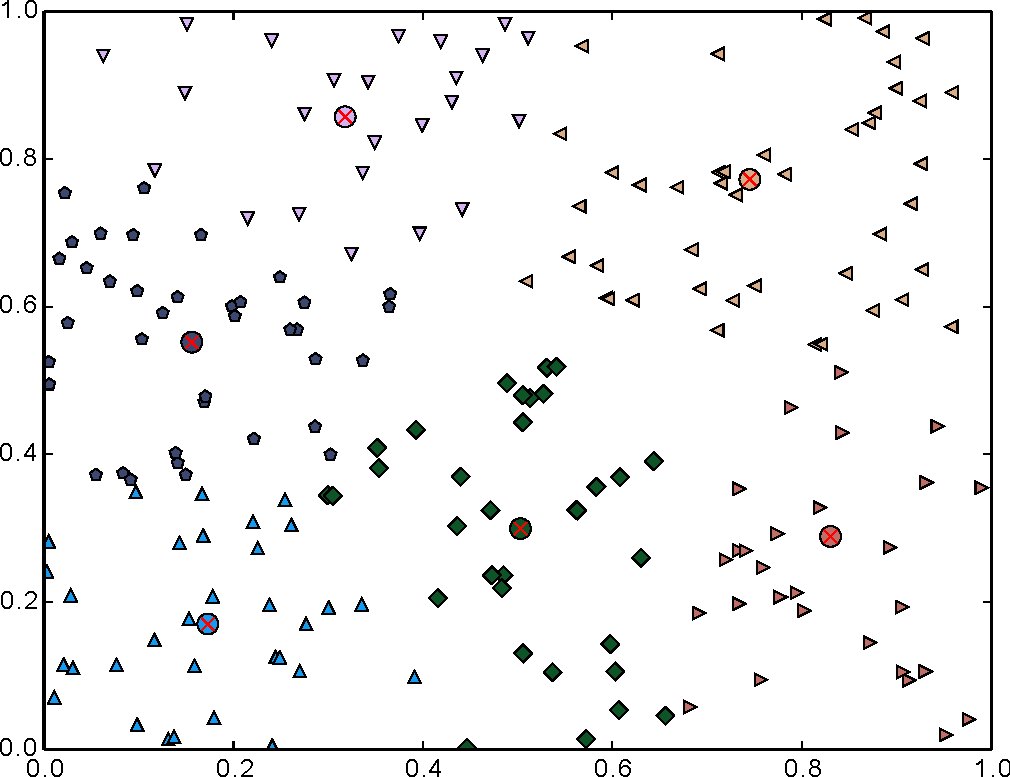
\includegraphics[width=0.7\linewidth]{./figure/kmean}
\caption{K-Mean classifier.}
\label{fig:interclass_variances}
\end{figure}

\section{Pattern recognition}
\label{sec:pattern_recognition}





\bibliography{reference}
\bibliographystyle{plain}

\end{document}